\documentclass[10pt,a4paper]{article}
\usepackage[natbibapa]{apacite} 
\usepackage{amsmath}
\usepackage{tikz}
\bibliographystyle{apacite}

\title{Investigation into the inner workings of Concept Learning and Decision Trees}
\author{ Adriaan Louw (53031377)}

\def\layersep{2.5cm}

\begin{document}

\maketitle

\tableofcontents

\section{Background}

\section{Perceptrons}
\subsection{What is a Perceptron}
A perceptrons is a unit that takes in inputs $x_i$ and weights $\omega_i$ and returns either -1 or 1 depending on whether the dot product of $x_i$ and $\omega_i$ is larger than some $k$.  

\begin{equation}
\label{percept}
o(x_i,...,x_n) =
\begin{cases}
 1 & \omega_1x_1 + ... + \omega_nx_n > k \\
-1 & otherwise \\ 
\end{cases}
\end{equation}

Neural networks can be built up our of perceptrons. These form a layer of nodes in the neural network and can be used to map various boolean functions

\subsection{Perceptron learning algorithm}
Gradient decent algorithm can be used to train the neural networks based on perceptrons. There needs to be an error function that defines the training error. The error can be fined as  

\begin{equation}
E(\vec{\omega}) = \frac{1}{2}\sum_{d \in D} (t_d-o_d)^2
\end{equation}

where $d$ is a training example in the training set $D$, $t_d$ is the target output for training example $d$ and $o_d$ is the output of the neural network for training example $d$.
 
Training neural networks consist of updating the weights of each of the nodes in the network based upon some training data. As in 

\begin{equation}
\label{perceptError}
\vec{\omega_i} \leftarrow \vec{\omega_i} + -\eta\bigtriangledown E(\vec{\omega})
\end{equation}

where $\vec{\omega}$ is the set of weights of the neural network, $\eta$ is the learning rate and $\bigtriangledown E(\vec{\omega})$ is the partial derivative of the Error function. The negative of the derivative is used to minimise the size of the error. In other words, the weights are updated each iteration such that the error becomes smaller until some minimum value is reached.


\begin{equation}
\begin{split}
\bigtriangledown E(\vec{\omega}) &= \frac{\delta}{\delta \omega_i} \frac{1}{2}\sum_{d \in D} (t_d-o_d)^2 \\
&=  \frac{1}{2}\sum_{d \in D} \frac{\delta}{\delta \omega_i}(t_d-o_d)^2 \\
&=  \frac{1}{2}\sum_{d \in D} 2(t_d - o_d) \frac{\delta}{\delta \omega_i}(t_d-o_d) \\
&=  \sum_{d \in D} (t_d - o_d) \frac{\delta}{\delta \omega_i}(t_d-o_d) \\
\end{split}
\end{equation}

Then using Equation \ref{percept} as a definition for $o_d$ we get

\begin{equation}
\label{full}
\begin{split}
\bigtriangledown E(\vec{\omega}) &= \sum_{d \in D} (t_d - o_d) \frac{\delta}{\delta \omega_i}(t_d-o_d) \\
&=  \sum_{d \in D} (t_d - o_d) \frac{\delta}{\delta \omega_i}(t_d-\vec{\omega}.\vec{x_d}) \\
&= -  \sum_{d \in D} (t_d - o_d)x_{id} \\
\end{split}
\end{equation}

Therefore combining equations \ref{perceptError} and \ref{full}

\begin{equation}
\vec{\omega_i} \leftarrow \vec{\omega_i} + \sum_{d \in D} (t_d - o_d)x_{id} 
\end{equation}

Each weight is updated by using the previous value of the weight plus the learning rate $\eta$ times the error for each weight and data point.

\subsection{Examples}
\subsubsection{Example 1}

Given boolean function $A \wedge B$. This gives can be represented by the truth table

\begin{tabular}{|c|c|c|}
\hline
$A$ & $B$ & $A\wedge B$ \\
\hline
-1 & -1 & -1 \\
-1 & 1 & -1 \\
1 & -1 & -1 \\
1 & 1 & 1 \\
\hline
\end{tabular}

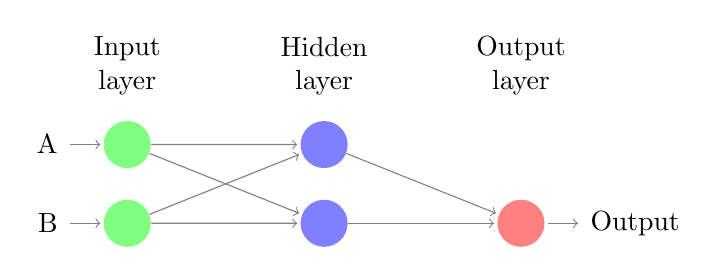
\begin{tikzpicture}[shorten >=1pt,->,draw=black!50, node distance=\layersep]
    \tikzstyle{every pin edge}=[<-,shorten <=1pt]
    \tikzstyle{neuron}=[circle,fill=black!25,minimum size=17pt,inner sep=0pt]
    \tikzstyle{input neuron}=[neuron, fill=green!50];
    \tikzstyle{output neuron}=[neuron, fill=red!50];
    \tikzstyle{hidden neuron}=[neuron, fill=blue!50];
    \tikzstyle{annot} = [text width=4em, text centered]

    % Draw the input layer nodes
    \node[input neuron, pin=left:A] (I-1) at (0,-0.5) {};
    \node[input neuron, pin=left:B] (I-2) at (0,-1.5) {};

    % Draw the hidden layer nodes
    \foreach \name / \y in {1,...,2}
        \path[yshift=0.5cm]
            node[hidden neuron] (H-\name) at (\layersep,-\y cm) {};

    % Draw the output layer node
    \node[output neuron,pin={[pin edge={->}]right:Output}, right of=H-2] (O) {};

    % Connect every node in the input layer with every node in the
    % hidden layer.
    \foreach \source in {1,...,2}
        \foreach \dest in {1,...,2}
            \path (I-\source) edge (H-\dest);

    % Connect every node in the hidden layer with the output layer
    \foreach \source in {1,...,2}
        \path (H-\source) edge (O);

    % Annotate the layers
    \node[annot,above of=H-1, node distance=1cm] (hl) {Hidden layer};
    \node[annot,left of=hl] {Input layer};
    \node[annot,right of=hl] {Output layer};
\end{tikzpicture}


We will need a network with 2 input nodes and 1 output node. 

The treshold 
\subsection{Limitations of Perceptrons}

A 2 layer percepron network can implement any boolean function. But no network of perceptrons can implement continuous functions. This is because of the nature of the perceptron, returning -1 or 1 depending on some threshold.

\citep{Michell2009}
\section{Backpropagation}
\subsection{Original Paper On Error Propagation}
\cite{rumel} is the first paper on error propagation.

\subsection{Most common form of Backpropagation}
\begin{enumerate}
\item Create network with $n_{in}$ inputs, $n_{hidden}$ hidden units, and $n_{out}$ output units
\item Initialise all weights to a small random number 
\item Until termination condition is reached
    \begin{enumerate}
    \item For each $\langle\vec{x},\vec{t}\rangle$ training example
         \begin{enumerate}
         \item Input instance $\vec{x}$ into network
         \item Compute output $o_u$ of every unit $u$ in network.
         \item For each output unit $k$ calculate its error term $\delta_k$
             \begin{equation}
             \delta_k \leftarrow o_k(1-o_k)(t-o_k)
             \end{equation}
         \item For each hidden unit h, calculate its error term $\delta_h$
             \begin{equation}
             \delta_h \leftarrow o_h(1-o_h)\sum_{k\in outputs} \omega_{kh}\delta_k
             \end{equation}
         \item Update each network weight $\omega_{ji}$
             \begin{equation}
             \omega_{ij} \leftarrow \omega_{ij} + \eta \delta_j x_{ji}
             \end{equation}                                          
         \end{enumerate}                 
    \end{enumerate}
\end{enumerate}

From \cite[p98]{Michell2009}

\subsection{Variants and extentions to Backpropagation}

\subsection{Question 3.4}

\subsection{Question 3.5}

For the play tennis example. We will use 6 input nodes ($x_1,...,x_6$). $x_1$ = Sky, $x_2$ = AirTemp, $x_3$ = Humidity, $x_4$ = Wind, $x_5$ = Water and $x_6$ = Forecast. There will be 6 hidden nodes ($h_1,...,h_6$) and one output node. We additionally have a training rate $\eta = 0.1$.

We need to represent these boolean states ad real numbers. Therefore the first value will be 0.1 and the second 0.9. 

Thus for Sky: Sunny = 0.1 and Rainy = 0.9 

For AirTemp: Warm = 0.1 and Cold = 0.9

For Humidity: Normal = 0.1 and High = 0.9

For Wind: Strong = 0.1 and Weak = 0.9

For Water: Warm = 0.1 and Cool = 0.9

For Forecast: Same = 0.1 and Change = 0.9 

Output layer will return 0.1 for No and 0.9 for Yes.

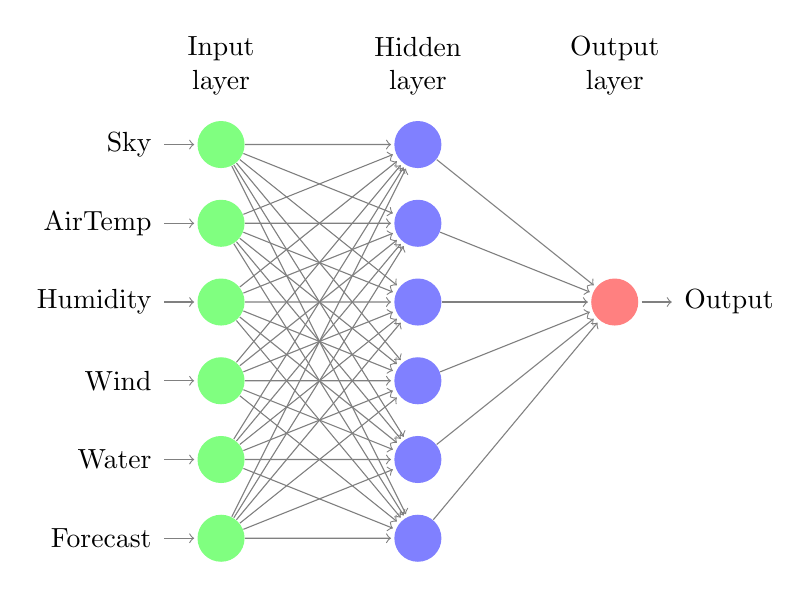
\begin{tikzpicture}[shorten >=1pt,->,draw=black!50, node distance=\layersep]
    \tikzstyle{every pin edge}=[<-,shorten <=1pt]
    \tikzstyle{neuron}=[circle,fill=black!25,minimum size=17pt,inner sep=0pt]
    \tikzstyle{input neuron}=[neuron, fill=green!50];
    \tikzstyle{output neuron}=[neuron, fill=red!50];
    \tikzstyle{hidden neuron}=[neuron, fill=blue!50];
    \tikzstyle{annot} = [text width=4em, text centered]

    % Draw the input layer nodes
    \node[input neuron, pin=left:Sky] (I-1) at (0,-0.5) {};
    \node[input neuron, pin=left:AirTemp] (I-2) at (0,-1.5) {};
    \node[input neuron, pin=left:Humidity] (I-3) at (0,-2.5) {};
    \node[input neuron, pin=left:Wind] (I-4) at (0,-3.5) {};
    \node[input neuron, pin=left:Water] (I-5) at (0,-4.5) {};
    \node[input neuron, pin=left:Forecast] (I-6) at (0,-5.5) {};

    % Draw the hidden layer nodes
    \foreach \name / \y in {1,...,6}
        \path[yshift=0.5cm]
            node[hidden neuron] (H-\name) at (\layersep,-\y cm) {};

    % Draw the output layer node
    \node[output neuron,pin={[pin edge={->}]right:Output}, right of=H-3] (O) {};

    % Connect every node in the input layer with every node in the
    % hidden layer.
    \foreach \source in {1,...,6}
        \foreach \dest in {1,...,6}
            \path (I-\source) edge (H-\dest);

    % Connect every node in the hidden layer with the output layer
    \foreach \source in {1,...,6}
        \path (H-\source) edge (O);

    % Annotate the layers
    \node[annot,above of=H-1, node distance=1cm] (hl) {Hidden layer};
    \node[annot,left of=hl] {Input layer};
    \node[annot,right of=hl] {Output layer};
\end{tikzpicture}

From \cite[p101]{Michell2009} we have the error 

\begin{equation}
E(\vec\omega)=\frac{1}{2}\sum_{k \in outputs}(t_k-o_k)^2
\end{equation}

and from \cite[p97]{Michell2009} 

\begin{equation}
o = \frac{1}{1+e^{-\vec\omega.\vec x} }
\end{equation}
\bibliography{mybib}
\end{document}
